\section{Introduction}
\label{sec:intro}
\begin{quote}
\textit{“All photographs are accurate. None of them is the truth.”} \hfill--- Richard Avedon
\end{quote}
Take a look at your favorite photos and recall how the real scene appeared at that moment. Those cherished images often suffer from various degradations such as noise, environmental effects, and compression artifacts, caused by the physical limitations of cameras, suboptimal conditions, or manual post-processing. This long standing problem has motivated extensive research in Image Restoration (IR), which aims to recover high quality images from low quality inputs. Over the years, numerous task-specific methods have been proposed for different degradations, such as denoising~\cite{zhang2023practical,chen2023masked}, relighting~\cite{liu2025dreamlight}, decompression~\cite{cheng2022optimizing}, etc. Although these methods achieve strong performance on individual restoration tasks, their task-specific nature limits their ability to generalize, making them less effective in handling diverse distortions in real-world scenarios.
\begin{figure}[t]
\begin{center}
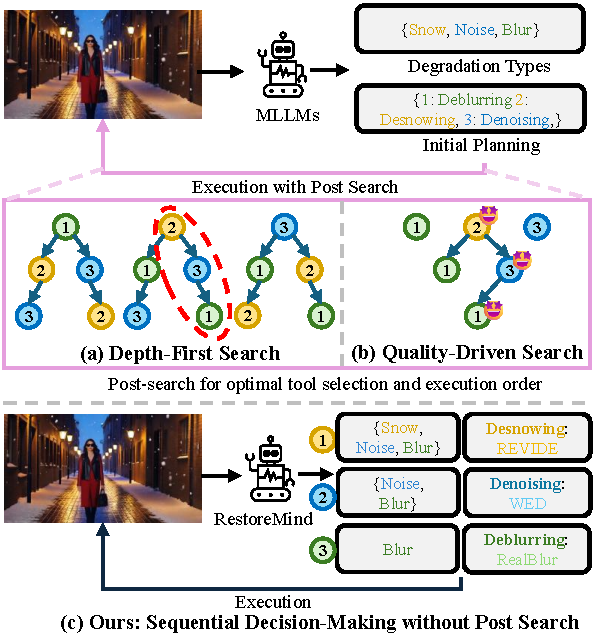
\includegraphics[width=1\linewidth]{fig/restoramind.pdf}
\end{center}
   \vspace{-0.5cm}
   \caption{}
   %$\hat{x}_0$ with different steps of  $\hat{x}_0$ prediction . \textbf{Prompts: } \emph{A white-haired girl in a pink sweater looks out a window in her bedroom.
\label{fig:pilot_study}
   \vspace{-0.5cm}

\end{figure}

% under unseen degradations in the wild.
% However, this strategy is highly sensitive to task order, and even minor changes in execution sequence can lead to significant performance degradation. Therefore, autonomously and efficiently coordinating expert models in real-world scenarios is essential for perceptual restoration.
To address this challenge, the All-in-One Image Restoration paradigm has attracted growing attention. It offers a unified framework capable of handling diverse and unknown degradations in the wild without requiring task-specific retraining. Recent studies have focused on simulating real-world degradations~\cite{peng2024towards}, proposing innovative architectural designs to balance multi-task knowledge~\cite{li2020knowledge}, and devising robust learning strategies to mitigate catastrophic forgetting~\cite{kirkpatrick2017overcoming}. However, like students facing difficult exam questions, these models still face challenges when generalizing beyond their training experience to out-of-distribution domains due to the inductive bias introduced by limited degradation combinations. For example, models trained on the degradation sequence of noise, blur, and JPEG compression fail to handle combinations like blur, JPEG compression, and noise, because compression and blurring alter the noise characteristics, making it smoother. There is also a trade-off between the number of degradation types and overall performance. In addition, their lack of fine-grained perception of degradation types and levels leads to unstable performance in the wild. Therefore, there is a pressing need to develop a system that can flexibly reason about various degradation types while adaptively handling them with task-specific knowledge.
% 在JPEG压缩/模糊之前添加噪声会改变噪声的特性，使其因压缩/模糊效果而变得更加平滑。相反，在噪声之前添加JPEG压缩/模糊则不会改变噪声的特性。

% 第三段讲基于VLM的agentic IR，引出我们的工作
% IR toolbox
Multimodal Large Language Models (MLLMs) have recently achieved remarkable breakthroughs in visual understanding and reasoning. Inspired by this progress, agentic IR are emerging under a new paradigm. Most existing pipelines follow a closed-loop search strategy~\cite{wu2025vtool}, which involves three stages:
(1) constructing a toolbox by integrating specialized restoration models that excel in their respective domains;
(2) using MLLMs for degradation reasoning and planning the execution sequence of tools from the toolbox; and
(3) recalibrating the planned route in (2) based on the restoration quality.
When the result is unsatisfactory, the system rolls back to (2) for replanning. In practice, such post-search mechanisms often suffer from substantial inefficiency when recalibrating an optimal execution order.
For instance, AgenticIR~\cite{zhu2024intelligent} takes about 63 minutes to restore an image with three degradation types using a toolbox of sixteen tools. The inference time grows exponentially as more IR tools are added to the toolbox and additional degradation types are considered, which significantly hinders its practical deployment. To overcome this limitation, we ask a fundamental question: Can we endow an MLLMs-powered agent with the capability to reason about degradations while adaptively utilizing restoration tools? In this paper, we present RestorMind, a novel agentic IR framework trained end-to-end with reinforcement learning to answer this question. The proposed method moves beyond merely reasoning about image degradations, advancing toward a new paradigm where models can actively employ and coordinate restoration tools to recover the image. This marks a fundamental shift in the cognitive mechanism of agentic IR systems, from passively applying multiple tools through trial and error to proactively reasoning about which tool to use and how to use it. Much like a child developing from unstructured experimentation to deliberate problem-solving, our approach empowers the model to think and act with intent, transforming image restoration from a reactive process into a reasoning-driven one.


% 我们的方法
RestoraMind formulates image restoration as a sequential decision-making process that jointly models degradation reasoning and tool selection. To achieve this, we initialize the agent with a degradation-aware VLLM~\cite{li2025q} as a cold start and train it end-to-end using reinforcement learning. At each state, the agent first predicts the degradation types of the distorted image and then adaptively selects one restoration tool from the toolbox for restoration. The predicted degradation types, the restored image, and the selected tool form a triplet that serves as the input for the next state, where the restored image functions as the observation. 
The agent switches to tools handling other degradation types once the previous degradation has been either resolved or remains after the reprocessing attempt. We encourage the agent to explore more effective tool execution sequences by penalizing decision routes that fail to restore all degradations within a fixed number of dialogue rounds with lower score. Besides the execution order, selecting the appropriate tool for each degradation type is equally crucial. Image restoration is inherently ill-posed, and different tools exhibit complementary performance when handling the same degradation type across different images. This observation motivates us to enable the agent to adaptively master the suitable tools for different images. To this end, we incorporate image statistical features into each state as auxiliary inputs to the VLLM. These low-level features provide structural cues that enable the VLLM to capture image priors and make more informed tool selections. For the reward function, we combine step-wise quality rewards with degradation-type rewards, which together encourage progressive restoration and mitigate capability forgetting, enabling seamless integration of degradation reasoning and tool selection. Extensive experiments validate that the proposed RestoraMind is intelligent in restoration reasoning and tool utilization, outperforming both All-in-One and existing agentic restoration models.


% RestoraMind formulates image restoration as a sequential decision-making process that jointly models degradation reasoning and tool selection. To achieve this, we initialize the agent with a degradation-aware VLLM as a cold start and train it end-to-end using reinforcement learning. At each state, the agent first predicts the degradation types of the distorted image and then adaptively selects one restoration tool from the toolbox for restoration. The predicted degradation types, the restored image, and the selected tool form a triplet that serves as the input for the next state, where the restored image functions as the observation. In subsequent states, the agent reasons about the remaining degradation types and assesses whether the tool used in the previous step has removed the corresponding degradation. When the degradation remains, the agent rolls back to the previous state and re-restores the original image or previous observation using an alternative tool of the same degradation type.
% The agent switches to tools handling other degradation types once the previous degradation has been either resolved or remains after the reprocessing attempt. When the agent fails to restore all degradations within a fixed number of dialogue rounds, it receives a low reward, encouraging exploration of more effective tool execution sequences in future iterations.
% Through this process, the agent gradually learns to organize restoration tools into the most effective order for different combinations of degradations. In addition to the execution order, selecting the appropriate tool for each degradation type is equally crucial.
% Image restoration is inherently ill-posed, and different tools often exhibit complementary performance even when addressing the same degradation type.
% This observation motivates us to enable the agent to adaptively master the most suitable tools for different images. To this end, we incorporate image statistical features into each state as auxiliary inputs to the VLLM. These low-level features provide structural cues that enable the VLLM to capture image priors and make more informed tool selections. For the reward function, we combine step-wise quality rewards with degradation-type rewards, which together encourage progressive restoration and mitigate capability forgetting, enabling seamless integration of degradation reasoning and tool selection.
% We cast the problem  of image restoration as a sequential decision-making process. In this paradigm, an agent learns to progressively restore a degraded image by iteratively applying operators from a predefined toolbox. The state of the environment is represented by the intermediate restoration result, which serves as a visual observation for our policy model, dubbed RestoraMind. Specifically, at each timestep, it perceives the current state, which includes the latest processed image and a history of its own past actions. Based on this state, RestoraMind first reasons about the image's degradation—assessing artifact types and severity, and then selects and executes a tool(action) from its toolbox. The environment's determinstic transition then yields the subsequent state, which is the newly refined image presented as the next observation. This immediate feedback loop is pivotal, enabling the policy to learn a direct mapping from action selection to its visual consequences—a capability absent in open-loop planning. We employ an end-to-end reinforcement learning framework to train it. The training is specifically designed to jointly optimize two coupled capabilities: the perceptual reasoning to assess the current image's degradation type, and the strategic selection of the subsequent optimal tool to apply. To achieve this goal, we have meticulously designed a composite reward function. This function innovatively optimizes for a dual objective: it not only rewards the step-wise improvement in final image quality, based on fidelity and perceptual metrics , but also directly incentivizes the agent's internal reasoning process by rewarding the accuracy of its degradation types. 


\begin{itemize}
% \vspace{-0.1in}
\item We propose RestoraMind, an MLLM-powered agent designed to restore images suffering from complex and unknown degradations. It follows a human-inspired problem-solving process that first reasons about the degradation types and then selects appropriate restoration tools for recovery.

\item We enhance the model’s tool-using intelligence through end-to-end reinforcement learning, which seamlessly integrates tool selection and degradation reasoning without requiring cold-start SFT or separate specialized restoration models.

\item Extensive experiments demonstrate that RestoraMind substantially accelerates the inference of agentic IR systems, achieving linear growth in inference time with respect to the number of degradation types, while significantly outperforming both All-in-One and existing agentic restoration models.

\end{itemize}


% We formally define the RestoraMind VLM as the central policy network of the agent, framing restoration as a sequential decision-making process solvable with reinforcement learning. The agent operates in an interactive, closed-loop system. At each timestep, it perceives the current state, which includes the latest processed image and a history of its own past actions. Based on this state, it selects and executes a tool (action) from its toolbox. The environment's deterministic transition provides the subsequent state, which crucially contains the new visual result of that action. This immediate feedback loop is pivotal, enabling the policy to learn a direct mapping from action selection to its visual consequences—a capability absent in open-loop planning. To optimize this VLM policy, we employ Group Relative Policy Optimization (GRPO), a state-of-the-art, critic-free RL algorithm. The policy is guided by a meticulously designed composite reward function. This function innovatively optimizes for a dual objective: it rewards not only the step-wise improvement in final image quality, based on fidelity and perceptual metrics , but also directly incentivizes the agent's internal reasoning process by rewarding the accuracy of its degradation types.


%restoring images with distortions 

% Like students facing difficult exam questions, these models tend to guess when uncertain, producing poor-quality restoration results. 

% Therefore, autonomously and efficiently coordinating expert models in real-world scenarios is essential for perceptual restoration.

% effectively handling unseen tasks and degradation types.

% pressing need to develop 
% generalize poorly to out-of-distribution domains
% synthetic image pairs that cannot fully simulate the complex real-world image degradations, 
% 第一段：请你仔细看看你相册中的照片，是否跟你眼睛看到的有差别。这是因为实际获取的图像通常会收到各种噪声，blur，光学传感器和后传输导致的变化。这种问题促使了image restoration近些年分裂出了非常多子任务，包括了denosing，deblur，religtinng和deratining等等。我们见证许多专家模型的诞生，such as~\cite (我们用的工具)。但是实际的图像面临复杂的损失，就像我们在用photoshop修图一样，难以用一个工具去修复图像。
 % 要定义的变量：specific IR tasks, low-quality (LQ), high-quality (HQ) task-specific knowledge in the network to deal with the corresponding restoration task

% 第二段：近些年all in one的模型获得了广泛关注，然后指出这类工作的不足。While current AiO IR networks are more effective than traditional ones designed for single degradations, training them is more challenging due to the potential conflicts among different optimization objectives [10, 28, 85]. Moreover, these models are typically limited to 3-5 specific tasks seen during training and struggle to generalize to unseen ones. When encountering degradations not included in training, they either require retraining or suffer from a large drop in the quality of recovered images. This hampers their practical application in real-world scenarios, where images are often affected by a wider range of degradations. 比喻，这类模型遇到不会的问题会给出Like students facing hard exam questions, large language models sometimes guess when uncertain, producing plausible yet incorrect statements instead of admitting uncertainty.

% This restricts their real-world application since it requires training individual models for each specific degradation and knowing the input degradation type to apply the relevant model.

% 第三段：VLM的引入% Large Multimodal Models (LMMs) have recently marked a pivotal moment in artificial intelligence, demonstrating remarkable success in comprehending and generating multimodal content [Team et al., 2023, Liu et al., 2024a, Wang et al., 2024a, Chen et al., 2025a]. This progress has fundamentally reshaped AI’s ability to bridge the cognitive gap between visual perception and linguistic abstraction. A key catalyst for this first wave of advancement has been the adaptation of language-centric reasoning mechanisms, most notably the Chain-of-Thought (CoT) paradigm [Wei et al., 2022, Kojima et al., 2022]. By decomposing complex problems into a sequence of textual reasoning steps, CoT has significantly elevated LMM performance on a wide array of multimodal tasks, including visual question answering [Zhang et al., 2023a, He et al., 2025a, Shen et al., 2025], visually-grounded mathematical problem-solving [Lu et al., 2023], and intricate narrative generation [Wu et al., 2024a]. In this established paradigm, which we term “Thinking about Images”, the visual modality primarily serves as a static, initial context. LMM first “sees” an image, encodes it into a fixed set of features, and then operates exclusively within the textual domain to conduct its reasoning. The image is the premise, but language is the exclusive medium of thought. While powerful, this text-centric approach has exposed a fundamental limitation: the semantic gap between the rich, continuous, and often ambiguous nature of the visual world and the discrete, symbolic structure of language [Li et al., 2022]. This initial, one-time encoding flattens the visual world into a static representation, creating a critical information bottleneck. Consequently, models often falter on tasks that demand deeper, iterative visual engagement, such as complex physical reasoning [Balazadeh et al., 2024], precise spatial manipulation [Gupta and Kembhavi, 2023], or long-horizon planning in interactive environments [Pahuja et al., 2025, Wang et al., 2025a].Now, a new revolution is quietly unfolding in multimodal reasoning. Models are evolving beyond merely thinking about images with text, towards a new paradigm where they can truly think with images. This represents a fundamental shift in the cognitive role of vision: from a passive, fixed input to a dynamic, manipulable cognitive workspace. Much like a human using a sketchpad, models are now being empowered to actively query, modify, and even generate new visual information as integral, intermediate steps within their reasoning process. This ability to form a “visual chain of thought” is not a mere extension of textual CoT, but a revolutionary step towards a more holistic and human-like form of cognition [Larkin and Simon, 1987]. We argue that this emerging paradigm, “Thinking with Images”, constitutes the next frontier for multimodal AI. It is defined by its core principle: to utilize visual representations as a form of manipulable and verifiable thought, thereby empowering models to actively see, manipulate, and reason with visual information as intermediate steps in a cognitive process. This survey provides the first comprehensive and systematic overview of this nascent and rapidly accelerating field. To structure this rapidly evolving landscape, we propose a conceptual framework that charts the progression of this paradigm through three stages of increasing cognitive autonomy. These stages represent the different mechanisms (the “How”) through which a model can achieve its visual reasoning goals (the “Why”): from acting as a “commander” that orchestrates external visual tools, to evolving into a “visual programmer” that generates code for tailored operations, and ultimately becoming a “visual thinker” capable of intrinsic imagination and simulation. This three-stage evolution will be detailed in Section 2. The proliferation of methods across these stages naturally raises a critical question that this survey seeks to answer:


% 第四段：Agentic model

% 第五段：我们的方法

% MoE issues: However, these methods suffer from high computational costs, increased inference complexity as the number of experts grows, and lack explicit degradation modeling, limiting adaptability to unseen or complex degradations. Prompt-based methods, like OneRestore [9], guide restoration using degradation prompts, integrating scene descriptors via cross-attention mechanisms for flexible and adaptive strategies. While effective, these methods rely on coarse prompts that fail to capture nuanced degradation characteristics and treat prompts as static inputs, limiting their ability to adapt to varying degradation intensities or specific requirements, leading to suboptimal results. % While current AiO IR networks are more effective than traditional ones designed for single degradations, training them is more challenging due to the potential conflicts among different optimization objectives [10, 28, 85]. Moreover, these models are typically limited to 3-5 specific tasks seen during training and struggle to generalize to unseen ones. When encountering degradations not included in training, they either require retraining or suffer from a large drop in the quality of recovered images. This hampers their practical application in real-world scenarios, where images are often affected by a wider range of degradations. % Despite their successes in certain scenarios, existing performant generative approaches [176, 211] can only handle limited degradation ranges, e.g., up to 4× upscaling, failing to recover extremely low-quality images with highly complex and diverse degradations in the wild. Moreover, SR specialist models are known to generalize poorly to out-of-distribution domains [23], let alone when applied on a different scaling factor. This is mainly due to heavy reliance on supervised learning on synthetic image pairs that cannot fully simulate the complex real-world image degradations, not to mention other domains, ranging from AI-generated imagery, scientific computing, to biomedical images. Last but not least, practically, users often demand highly specific workflows, e.g., only denoising, 4K upscaling, or prioritizing high fidelity over perceptual quality, and a one-size-fits-all system that can flexibly adapt to satisfy diverse requirements and application scenarios is in pressing need. % Despite notable advancements, persistent challenges remain: current models still struggle with handling complex and compounded degradations, suffer from computational inefficiencies, and do not generalize well in real-world scenarios. % Existing All-in-One image restoration methods often fail to simultaneously perceive degradation types and severity levels, overlooking the importance of fine-grained quality perception, 导致了模型面对超出out-of-distribution domains就会猜测结果，从而带来poor restoration quality. Like students facing hard exam questions, large language models sometimes guess when uncertain, producing plausible yet incorrect statements instead of admitting uncertainty.